\section{A Functional Framework for Networked XR}\label{sec:framework}

The atlas labels every paper by the networking problem it addresses and by the content it carries. These
labels are precise, but \nxrNCatProb{} problems and \nxrNCatCont{} content types are too many to reason
about together, and they mix levels: ``latency'' is a property, ``caching'' a mechanism and
``holographic communication'' an application. We therefore group them by \emph{function}, the job a
part of the system performs in the loop between the user's body and the content they perceive. A function
is defined by a design question that any networked XR system must answer, whatever its medium or access
network. \Cref{fig:architecture} places the six functions on a reference architecture, and
\cref{tab:framework} lists the atlas categories that each function contains.

\begin{figure}[t]
\centering
\begin{tikzpicture}[font=\sffamily\scriptsize,
  tier/.style={draw=black!15,fill=black!3,rounded corners=3pt,minimum width=3.75cm,minimum height=5.85cm,anchor=north},
  tierhead/.style={font=\sffamily\footnotesize\bfseries,text=black!75},
  comp/.style={draw=black!55,fill=white,rounded corners=2pt,align=center,minimum height=7.5mm,text width=3.2cm,inner sep=1.5pt,line width=0.5pt},
  fn/.style={rounded corners=1.2pt,font=\sffamily\tiny\bfseries,inner sep=1.3pt,text=black,anchor=south west,yshift=0.4pt},
  up/.style={-{Stealth[length=1.6mm]},line width=0.6pt,black!65,dashed},
  down/.style={-{Stealth[length=1.6mm]},line width=0.9pt,black!75},
  ctl/.style={{Stealth[length=1.4mm]}-{Stealth[length=1.4mm]},line width=0.6pt,black!55,densely dotted}]
  \def\X{{1.875,6.075,10.275,14.475}}
  \foreach \x/\name in {1.875/XR device,6.075/Access network,10.275/Edge,14.475/Cloud and origin}{
    \node[tier] at (\x,0) {};
    \node[tierhead] at (\x,-0.3) {\name};}
  % Row 1: uplink and interaction
  \node[comp] (sens) at (1.875,-1.3) {Sensors: pose, gaze,\\camera, capture};
  \node[comp] (ul)   at (6.075,-1.3) {Uplink: OFDMA,\\configured grants};
  \node[comp] (rend) at (10.275,-1.3) {Remote or split renderer,\\AR inference};
  \node[comp] (app)  at (14.475,-1.3) {Application server,\\world state, economy};
  % Row 2: downlink content
  \node[comp] (dec)  at (1.875,-2.5) {Decoder, local render,\\reprojection, display};
  \node[comp] (dl)   at (6.075,-2.5) {Downlink: mmWave, THz,\\RIS, Wi-Fi 6/7};
  \node[comp] (cache) at (10.275,-2.5) {Edge cache and\\prefetcher};
  \node[comp] (enc)  at (14.475,-2.5) {Encoder and store: tiles,\\V-PCC, MIV, splats};
  % Row 3: control and transport
  \node[comp] (pred) at (1.875,-3.7) {Viewport and motion\\predictor, ABR client};
  \node[comp] (sch)  at (6.075,-3.7) {XR-aware scheduler,\\slices, RIC controllers};
  \node[comp] (state) at (10.275,-3.7) {Session state, relay,\\interest management};
  \node[comp] (cdn)  at (14.475,-3.7) {CDN, multicast, QUIC,\\WebRTC, L4S, FEC};
  % Row 4: physical coupling
  \node[comp] (hap)  at (1.875,-4.9) {Haptic device,\\teleoperation master};
  \node[comp] (twin) at (10.275,-4.9) {Digital twin,\\teleoperation proxy};
  \node[draw=black!40,fill=white,rounded corners=2pt,align=center,text width=3.2cm,minimum height=7.5mm,inner sep=1.5pt] (peers) at (6.075,-4.9)
     {Other users and remote\\machines (robot, plant)};
  % Flows
  \draw[up] (sens) -- (ul); \draw[up] (ul) -- (rend); \draw[up] (rend) -- (app);
  \draw[down] (enc) -- (cache); \draw[down] (cache) -- (dl); \draw[down] (dl) -- (dec);
  \draw[down] (rend.south west) -- (dl.north east);
  \draw[ctl] (pred) -- (sch); \draw[ctl] (sch) -- (state); \draw[ctl] (state) -- (cdn);
  \draw[ctl] (hap) -- (peers); \draw[ctl] (peers) -- (twin); \draw[ctl] (twin) -- (state);
  % Function tags
  \node[fn,fill=encode!30,draw=encode!80!black] at (enc.north west) {1 Encode};
  \node[fn,fill=encode!30,draw=encode!80!black] at (sens.north west) {1 Encode};
  \node[fn,fill=anticipate!30,draw=anticipate!80!black] at (pred.north west) {2 Anticipate};
  \node[fn,fill=anticipate!30,draw=anticipate!80!black] at (cache.north west) {2 Anticipate};
  \node[fn,fill=compute!30,draw=compute!80!black] at (rend.north west) {3 Compute};
  \node[fn,fill=compute!30,draw=compute!80!black] at (dec.north west) {3 Compute};
  \node[fn,fill=provision!25,draw=provision!80!black] at (ul.north west) {4 Provision};
  \node[fn,fill=provision!25,draw=provision!80!black] at (dl.north west) {4 Provision};
  \node[fn,fill=provision!25,draw=provision!80!black] at (sch.north west) {4 Provision};
  \node[fn,fill=provision!25,draw=provision!80!black] at (cdn.north west) {4 Provision};
  \node[fn,fill=connect!35,draw=connect!80!black] at (state.north west) {5 Connect};
  \node[fn,fill=connect!35,draw=connect!80!black] at (twin.north west) {5 Connect};
  \node[fn,fill=connect!35,draw=connect!80!black] at (hap.north west) {5 Connect};
  \node[fn,fill=connect!35,draw=connect!80!black] at (app.north west) {5 Connect};
  % Assure band
  \node[draw=assure!80!black,fill=assure!10,rounded corners=2pt,minimum width=16.35cm,minimum height=5mm,anchor=south,
        font=\sffamily\scriptsize] at (8.175,0.12)
     {\textbf{6 Assure}\enspace across the whole loop: QoE and cybersickness, motion-to-photon and tail latency, privacy of pose and traffic, authentication};
  % Legend
  \begin{scope}[shift={(13.0,-4.75)},font=\sffamily\tiny]
    \draw[up] (0,0.22) -- (0.55,0.22) node[right,text=black]{uplink};
    \draw[down] (0,-0.05) -- (0.55,-0.05) node[right,text=black]{downlink content};
    \draw[ctl] (0,-0.32) -- (0.55,-0.32) node[right,text=black]{control and shared state};
  \end{scope}
\end{tikzpicture}
\caption{Reference architecture of a networked XR system, with the six functions placed where they act.
Rows read left to right as the uplink of pose and captured media, right to left as the downlink of
content, and as control and shared state that couple users and remote machines. The same function often
acts at several tiers: anticipation runs both on the device (prediction) and at the edge (caching), and
computation is split between device and edge.}\label{fig:architecture}
\end{figure}

\paragraph{The six functions.}
\begin{description}[leftmargin=0pt,itemsep=2pt,font=\normalfont\bfseries]
  \item[Encode] (\cref{sec:encode}). \emph{What representation of the scene travels, and how is it
        compressed?} Projections and tiling of 360-degree video, point clouds and meshes, multi-view
        video, neural scene representations, holograms and haptic signals.
  \item[Anticipate] (\cref{sec:anticipate}). \emph{What will the user need next, and how is it delivered
        in time?} Viewport-adaptive streaming, head, gaze and 6DoF motion prediction, and caching and
        prefetching.
  \item[Compute] (\cref{sec:compute}). \emph{Where does each stage of perception and rendering run, and
        how is the added delay budgeted and hidden?} Offloading, remote and split rendering, AR inference
        at the edge, motion-to-photon budgets, reprojection and device energy.
  \item[Provision] (\cref{sec:provision}). \emph{How do radio, scheduling, transport and architecture
        supply the rate, delay and reliability required?} Resource allocation, mmWave, terahertz,
        reconfigurable surfaces and Wi-Fi, congestion control and loss resilience, and 6G and metaverse
        architectures.
  \item[Connect] (\cref{sec:connect}). \emph{How are several people and remote machines kept consistent
        and responsive?} Multi-user synchronisation, avatars, haptic teleoperation, holographic
        telepresence and digital twins.
  \item[Assure] (\cref{sec:assure}). \emph{How do we know the result is good enough, and safe?} QoE
        measurement and modelling, traffic characterisation, and security, privacy and trust.
\end{description}

Three properties make this grouping useful. First, it is \emph{exhaustive}: every networking problem in
the atlas codebook except the residual ``other'' (\nxrNProbOther{} papers) belongs to exactly one
function, and every specific content type has a natural home. Second, the functions are \emph{ordered
along the loop}. Encoding and anticipation decide what is sent, computation and provisioning decide where
and how, and connection and assurance concern the people at the ends. Third, each function has a
\emph{characteristic evidence profile} (\cref{tab:framework}). The functions that build systems
(compute, connect) are tested on real testbeds far more often than those that optimise models
(provision, encode). The same gap therefore recurs in different words across the sections that follow,
and Section~\ref{sec:synthesis} returns to it.

\begin{table}[t]
\centering\small
\caption{The six functions, the atlas categories they contain and their evidence profile. Papers: primary
problem label. Share: percentage of all papers in 2017--19 and in 2022--24. Real: evaluated on a real
network or testbed, with or without users. Sim.: simulation or analysis only.}\label{tab:framework}
\setlength{\tabcolsep}{4pt}
\begin{tabularx}{\linewidth}{@{}>{\raggedright\arraybackslash}p{1.6cm}>{\raggedright\arraybackslash}X>{\raggedright\arraybackslash}p{3.0cm}rcrr@{}}
\toprule
Function & Networking problems (atlas cells) & Main content types & Papers & Share 17--19 $\to$ 22--24 & Real & Sim.\\
\midrule
\textcolor{encode!80!black}{\textbf{Encode}} & Compression and coding & Volumetric, holographic, haptic & \fnEncodeN{} & \fnEncodeEarly{} $\to$ \fnEncodeLate{} & \fnEncodeReal{} & \fnEncodeSimAna{}\\
\textcolor{anticipate!80!black}{\textbf{Anticipate}} & Rate adaptation and streaming; viewport and motion prediction; caching and prefetching & 360-degree video, volumetric & \fnAnticipateN{} & \fnAnticipateEarly{} $\to$ \fnAnticipateLate{} & \fnAnticipateReal{} & \fnAnticipateSimAna{}\\
\textcolor{compute!70!black}{\textbf{Compute}} & Offloading and remote rendering; latency & Rendered frames, AR overlays & \fnComputeN{} & \fnComputeEarly{} $\to$ \fnComputeLate{} & \fnComputeReal{} & \fnComputeSimAna{}\\
\textcolor{provision!80!black}{\textbf{Provision}} & Resource allocation; wireless link design; architecture and vision & XR traffic in general & \fnProvisionN{} & \fnProvisionEarly{} $\to$ \fnProvisionLate{} & \fnProvisionReal{} & \fnProvisionSimAna{}\\
\textcolor{connect!80!black}{\textbf{Connect}} & Multi-user synchronisation; tactile and haptic transport; holographic communication & Avatars, haptic, holographic, digital twins & \fnConnectN{} & \fnConnectEarly{} $\to$ \fnConnectLate{} & \fnConnectReal{} & \fnConnectSimAna{}\\
\textcolor{assure!80!black}{\textbf{Assure}} & QoE measurement and modelling; security, privacy and trust & All & \fnAssureN{} & \fnAssureEarly{} $\to$ \fnAssureLate{} & \fnAssureReal{} & \fnAssureSimAna{}\\
\bottomrule
\end{tabularx}
\end{table}

\paragraph{How functions and content combine.} The two labelling dimensions are not independent, and
their dependence shows where the field's attention has and has not gone (\cref{fig:heatmap}). The
strongest associations are definitional and confirm the labels. Rate adaptation is studied mostly for
360-degree video (\nxrXObsRateAdaptationStreamingVideoThreeSixty{} papers against
\nxrXExpRateAdaptationStreamingVideoThreeSixty{} expected under independence), tactile transport for
haptic signals, and multi-user synchronisation for avatars. The informative cells are the weak ones.
Resource allocation for volumetric content holds \nxrXObsResourceAllocationVolumetricPointcloud{} papers
against \nxrXExpResourceAllocationVolumetricPointcloud{} expected, and offloading for avatars and social
state \nxrXObsOffloadingRemoteRenderingAvatarsSocialState{} against
\nxrXExpOffloadingRemoteRenderingAvatarsSocialState{}. QoE work rarely involves an edge deployment
(\nxrXObsQoeMeasurementModellingEdgeFog{} against \nxrXExpQoeMeasurementModellingEdgeFog{}), and
multi-user synchronisation over 5G is equally rare
(\nxrXObsMultiuserSynchronisationFiveGCellular{} against \nxrXExpMultiuserSynchronisationFiveGCellular{}).
The content types that the field now calls its future, volumetric and social, are the ones its
allocation and offloading machinery has least often been applied to.

\begin{figure}[t]
\centering
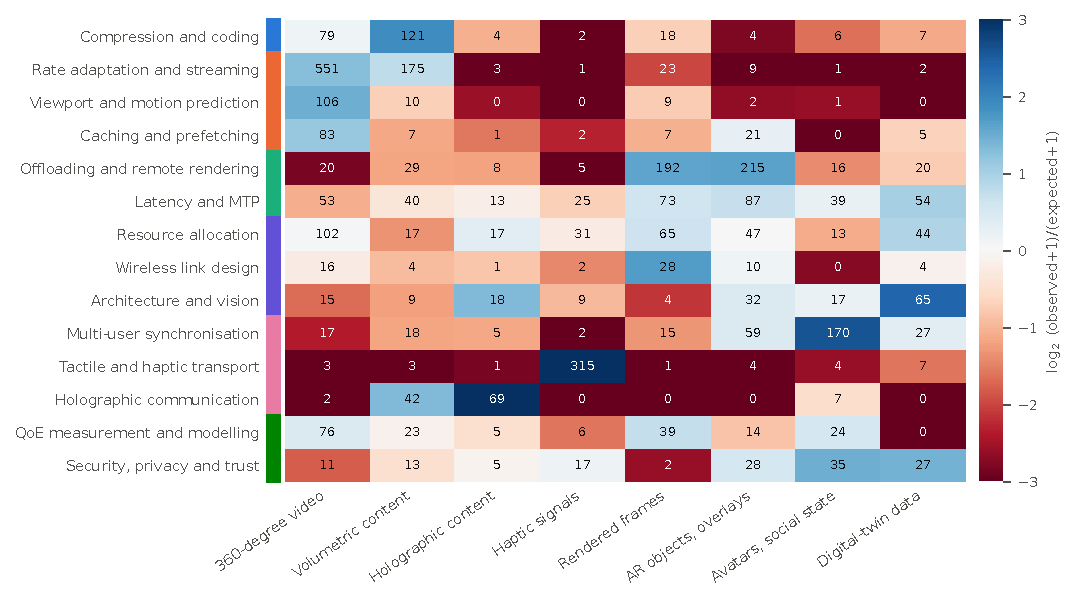
\includegraphics[width=0.86\linewidth]{fig_heatmap}
\caption{Networking problem (rows, grouped by function) against content type (columns). Numbers are
papers. Colour is $\log_2$ of observed over expected counts under independence: blue cells hold more
papers than expected and red cells fewer. ``XR traffic in general'' is omitted.}\label{fig:heatmap}
\end{figure}
